Pour comprendre pourquoi l'études des fractions continues multidimentionnels est intéressante, nous allons donner deux chemins qui y mênnent.
Le premier montre une approche géométrique du dévellopement en fraction continue dans le plan, qui est ensuite simple d'imaginer dans l'espace.
La seconde commence avec un autre objet de la théorie dynamique, les échanges d'interval.

\subsection{Cas de la dimension 1}

Soit $x \in ]0;1[$ et $e_1=(1,0)$ $e_2=(0,1)$ la base canonique de $\mathbb{R}^2$,
On note $D$ la demi-droite passant par $(0;0)$ et $X=(x;1)$. Comment former une suite de coefficient directeur rationnel de droite s'approchant de $D$ ?

Nous avons $X=xe_1+e_2=x(e_1+\frac{1}{x}e_2)=x(e_1+[\frac{1}{x}]e_2+\{\frac{1}{x}\}e_2)$
On pose donc $e_3=e_1+[\frac{1}{x}]e_2$ et nous avons $X=x(T(x) e_2+e_3)$ avec $T(x)=\{\frac{1}{x}\}$

Nous avons donc une seconde base $e_2$ et $e_3$ qui décrit aussi la droite $D$. Nous pouvons interpréter $e_3$ comme le premier point sur le réseau $\mathbb{Z}^2$ en dessous de l'intersection entre $D$ et la droite $\lambda e_2 +e_1$.
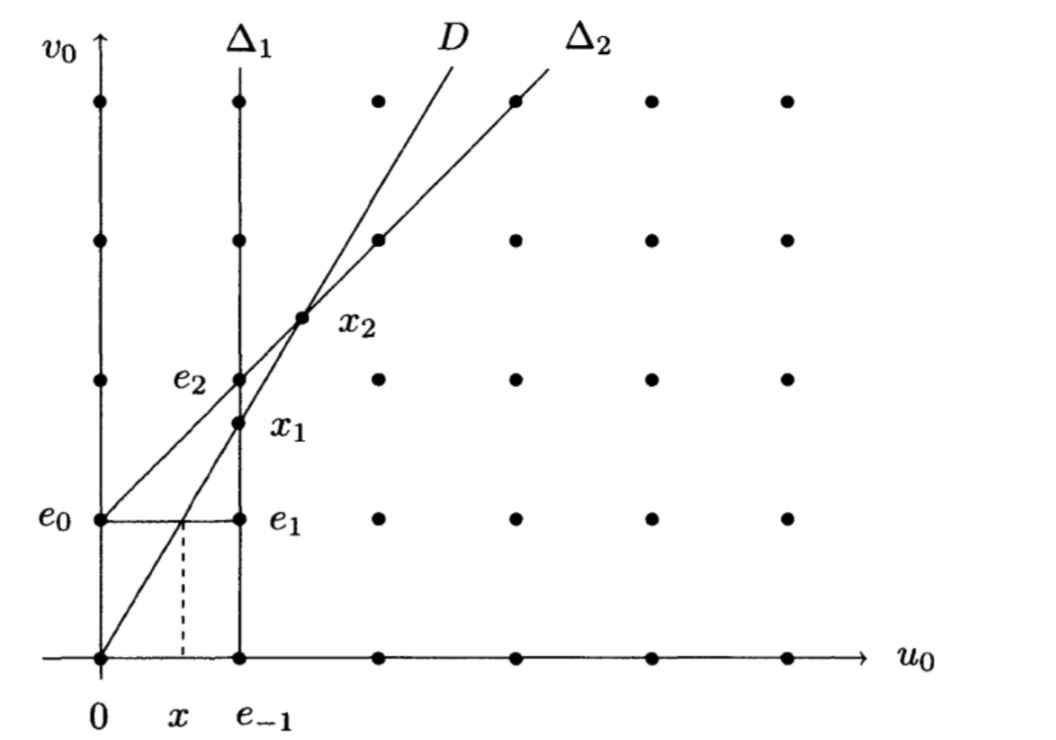
\includegraphics[width=16cm]{Image/ReseauDroite.png}
Nous pouvons alors itérer le processus avec $e_{n+1}=e_{n-1}+[\frac{1}{T^{n-1}(x)}]e_n$

Nous avons donc une suite de base $(e_n;e_{n+1})$ avec pour matrice de changement de base $P_n=
\begin{pmatrix}
   0 & 1 \\
   1 & [\frac{1}{T^{n-1}x}]
\end{pmatrix}$
En écrivant $e_{n+2}=(p_n;q_n)\in \mathbb{Z}^2$ nous avons:
$P_1...P_n=
\begin{pmatrix}
  p_{n-1} & p_n \\
  q_{n-1} & q_n
\end{pmatrix}$

Finalement nous avons $x=\frac{p_{n-1}T^n {x}+p_n}{q_{n-1}T^n x+q_{n-1}}$ pour tout $n$.

Pour généraliser cette construction, nous pouvons prendre deux réels $x,y$ compris entre $0$ et $1$, et soit $D$ la droite passant par $0$ et $x,y,1$. En partant de la base euclidienne habituel, nous cherchons une suite de trois vecteurs formant une base tel que les matrices de passages appartient à $SL_n(\mathbb(Z))$, le point $x,y,1$ soit une combinanison linéaire positive de ces trois vecteurs, et que ces trois vecteurs convergent dans un certain sens vers la droite $D$.
\subsection{Echange d'interval}
